\subsection{Visualizzazione mobile}

\par L'applicazione è progettata per essere utilizzata anche su dispositivi mobili, assicurando una buona esperienza utente su schermi touch screen di piccole dimensioni.

\begin{figure}[H]
  \centering
  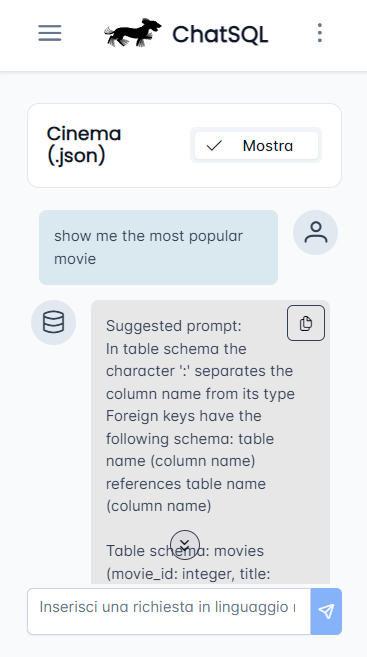
\includegraphics[width=0.50\textwidth]{assets/mobile.png}
  \caption{Versione mobile dell'applicazione}
\end{figure}

\par Per ottimizzare la navigazione sui dispositivi mobili, il menu principale è nascosto e può essere aperto cliccando sull'icona a tre linee 
\includegraphics[height=1.2em]{assets/dd_burger_menu.png} in alto a sinistra. Le pagine occupano l'intero schermo, per offrire il massimo spazio possibile al contenuto principale.
\par Per liberare spazio, i pulsanti di login e delle impostazioni di sistema sono stati nascosti e sono accessibili tramite un menu a tendina. Il menu si apre ciccando sull'icona con i tre puntini 
\includegraphics[height=1.2em]{assets/dd_kebab_menu.png} situata in alto a destra.